\documentclass[12pt]{standalone}
\usepackage{tikz,mathpazo }
\begin{document}
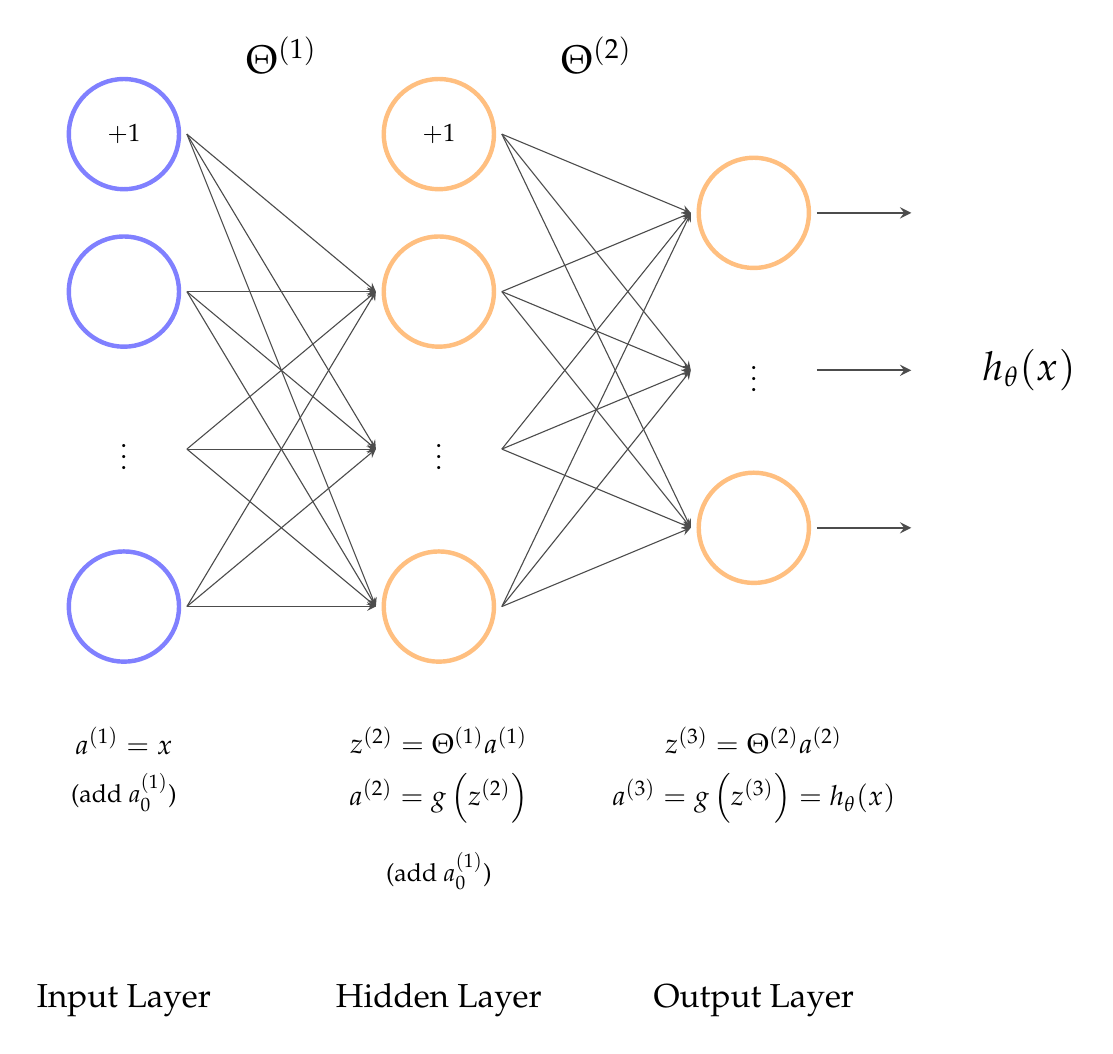
\begin{tikzpicture}[scale=2]
    \foreach \y in {1, 3, 4}{ \draw[blue!50, ultra thick] (0, \y) circle (0.35); }
    \foreach \y in {1, 3, 4}{ \draw[orange!50, ultra thick] (2, \y) circle (0.35); }
    \foreach \y in {1.5, 3.5}{ \draw[orange!50, ultra thick] (4, \y) circle (0.35); }
    \foreach \x in {1, 2, 3, 4}{%
        \foreach \y in {1, 2, 3}{ \draw[black!70, thin, -stealth] (0.4, \x) -- (1.6, \y); }
    }
    \foreach \x in {1, 2, 3, 4}{%
        \foreach \y in {1.5, 2.5, 3.5}{ \draw[black!70, thin, -stealth] (2.4, \x) -- (3.6, \y); }
    }
    \foreach \y in {1.5, 2.5, 3.5}{ \draw[black!70, -stealth, thick] (4.4, \y) -- (5, \y); }

    \draw (0, 2) node {$\vdots$};
    \draw (2, 2) node {$\vdots$};
    \draw (4, 2.5) node {$\vdots$};

    \foreach \x in {1, 2} {%
        \draw (\x+\x-2, 4) node {\small $+1$};
        \draw (\x+\x-1, 4.5) node {\Large $\Theta^{(\x)}$};
    }
    \draw (5.75, 2.5) node {\Large $h_\theta(x)$};
    \draw (0, 0) node [above]{$a^{(1)} = x$};
    \draw (0, 0) node [below]{\small (add $a_0^{(1)}$)};
    \draw (2, 0) node [above]{$z^{(2)}=\Theta^{(1)}a^{(1)}$};
    \draw (2, 0) node [below]{$a^{(2)}=g\left(z^{(2)}\right)$};
    \draw (2, -0.5) node [below]{\small (add $a_0^{(1)}$)};
    \draw (4, 0) node [above]{$z^{(3)}=\Theta^{(2)}a^{(2)}$};
    \draw (4, 0) node [below]{$a^{(3)}=g\left(z^{(3)}\right)=h_\theta(x)$};

    \draw (0, -1.5) node {\large Input Layer};
    \draw (2, -1.5) node {\large Hidden Layer};
    \draw (4, -1.5) node {\large Output Layer};
\end{tikzpicture}
\end{document}
